% =========================================================
% CHAPTER III
% SOFTWARE REQUIREMENT SPECIFICATION
% =========================================================

\chapter{ĐẶC TẢ YÊU CẦU PHẦN MỀM}


% =========================================================
% 1. TỔNG QUAN SẢN PHẨM
% =========================================================

\section{Tổng quan sản phẩm}

Nền tảng kết nối cộng đồng nhiếp ảnh phim với các dịch vụ phòng tối và
phòng chụp là một hệ thống được thiết kế để kết nối Photographer với
Service Provider cung cấp phòng tối, phòng chụp, thiết bị và các dịch vụ
hỗ trợ.

Hệ thống cho phép Photographer tìm kiếm, xem thông tin và đặt các không
gian dịch vụ. Người dùng có thể lựa chọn thời gian, thiết bị đi kèm,
thực hiện thanh toán và theo dõi trạng thái booking.

Service Provider có thể quản lý hồ sơ, không gian sáng tạo, thiết bị,
gói dịch vụ, booking và workshop trên cùng một nền tảng.

Administrator chịu trách nhiệm quản lý người dùng, quản lý Service
Provider, phê duyệt đăng ký Service Provider và theo dõi các giao dịch
trong hệ thống.

\begin{figure}[H]
	\centering
	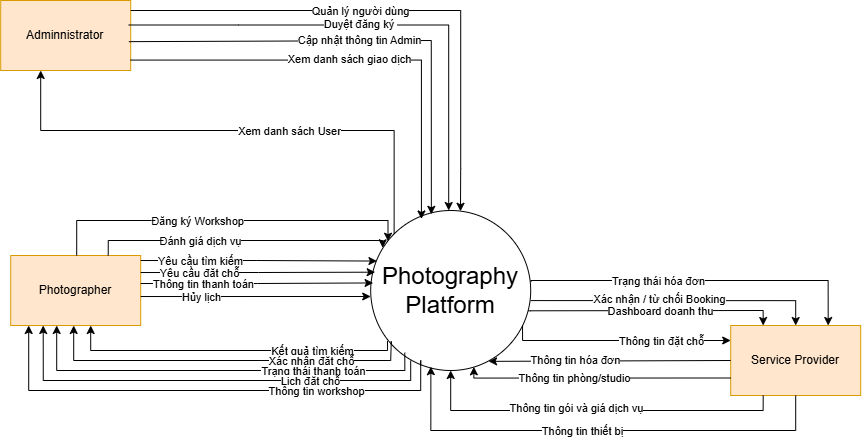
\includegraphics[width=\textwidth]{images/2.png}
	\caption{Sơ đồ ngữ cảnh của hệ thống}
	\label{fig:context-diagram}
\end{figure}


% =========================================================
% 2. YÊU CẦU NGƯỜI DÙNG
% =========================================================

\section{Yêu cầu người dùng}


\subsection{Actor}

Hệ thống gồm ba actor chính:

\begin{table}[H]sub
	\centering
	\caption{Các actor của hệ thống}
	\label{tab:actors}
	\begin{tabular}{|c|p{3.2cm}|p{8.2cm}|}
		\hline
		\textbf{\#} & \textbf{Actor} & \textbf{Mô tả} \\
		\hline
		
		1 &
		Photographer &
		Người dùng chính của hệ thống, có thể quản lý hồ sơ cá nhân, tìm kiếm
		dịch vụ, đặt chỗ, thanh toán, xem lịch sử booking và đăng ký workshop. \\
		\hline
		
		2 &
		Service Provider &
		Đơn vị cung cấp dịch vụ, có thể quản lý hồ sơ, không gian sáng tạo,
		thiết bị, gói dịch vụ, booking và workshop của mình. \\
		\hline
		
		3 &
		Administrator &
		Người quản trị hệ thống, có quyền quản lý người dùng, Service Provider,
		phê duyệt Service Provider và theo dõi giao dịch. \\
		\hline
		
	\end{tabular}
\end{table}


\subsection{Use Case}


\subsubsection{Sơ đồ Use Case}

\begin{figure}[H]
	\centering
	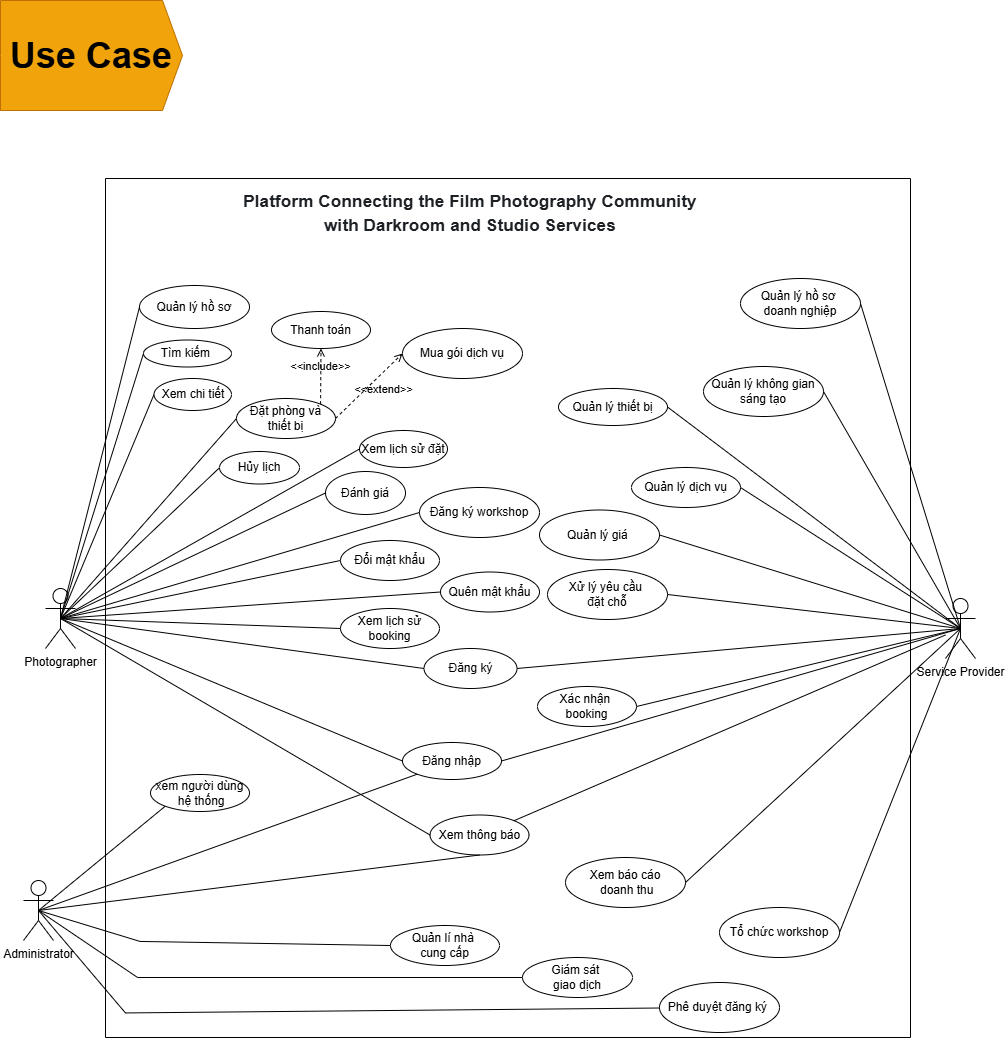
\includegraphics[width=\textwidth]{images/3.png}
	\caption{Sơ đồ Use Case của hệ thống}
	\label{fig:use-case-diagram}
\end{figure}

\newpage 

\subsubsection{Mô tả Use Case}

% =========================================================
% DANH SÁCH 34 USE CASE
% =========================================================

\setlength{\LTleft}{0pt}
\setlength{\LTright}{0pt}
\renewcommand{\arraystretch}{1.3}

\begin{longtable}{
		|>{\raggedright\arraybackslash}p{1.0cm}|
		>{\raggedright\arraybackslash}p{2.5cm}|
		>{\raggedright\arraybackslash}p{6.0cm}|
		>{\raggedright\arraybackslash}p{3.0cm}|
	}
	
	\caption{\raggedright Danh sách 34 Use Case của hệ thống}
	\label{tab:34-usecase}\\
	
	\hline
	
	\textbf{ID} &
	\textbf{Tên Use Case} &
	\textbf{Mô tả} &
	\textbf{Actor} \\
	
	\hline
	\endfirsthead
	
	\hline
	
	\textbf{ID} &
	\textbf{Tên Use Case} &
	\textbf{Mô tả} &
	\textbf{Actor} \\
	
	\hline
	\endhead
	
	UC01 &
	Đăng ký tài khoản Photographer &
	Cho phép Photographer tạo tài khoản mới. &
	Photographer \\
	
	\hline
	
	UC02 &
	Đăng nhập &
	Xác thực thông tin đăng nhập và truy cập hệ thống. &
	Photographer \\
	
	\hline
	
	UC03 &
	Đăng xuất &
	Cho phép người dùng đăng xuất khỏi hệ thống. &
	Photographer \\
	
	\hline
	
	UC04 &
	Quên mật khẩu &
	Cho phép người dùng thực hiện quy trình khôi phục mật khẩu khi quên mật khẩu. &
	Photographer \\
	
	\hline
	
	UC05 &
	Đổi mật khẩu &
	Cho phép Photographer thay đổi mật khẩu tài khoản. &
	Photographer \\
	
	\hline
	
	UC06 &
	Quản lý hồ sơ cá nhân &
	Cho phép Photographer xem và cập nhật thông tin hồ sơ cá nhân. &
	Photographer \\
	
	\hline
	
	UC07 &
	Tìm kiếm Creative Space &
	Cho phép Photographer tìm kiếm các Creative Space theo nhu cầu. &
	Photographer \\
	
	\hline
	
	UC08 &
	Xem chi tiết Creative Space &
	Hiển thị thông tin chi tiết của Creative Space được lựa chọn. &
	Photographer \\
	
	\hline
	
	UC09 &
	Đặt chỗ &
	Cho phép Photographer lựa chọn dịch vụ, thời gian và thực hiện đặt chỗ. &
	Photographer \\
	
	\hline
	
	UC10 &
	Xem chi tiết Booking &
	Hiển thị thông tin chi tiết của một Booking đã được tạo. &
	Photographer \\
	
	\hline
	
	UC11 &
	Hủy Booking &
	Cho phép Photographer hủy Booking theo trạng thái hợp lệ của Booking. &
	Photographer \\
	
	\hline
	
	UC12 &
	Xem lịch sử Booking &
	Cho phép Photographer xem danh sách các Booking đã thực hiện. &
	Photographer \\
	
	\hline
	
	UC13 &
	Xem hóa đơn &
	Cho phép Photographer xem thông tin hóa đơn liên quan đến Booking. &
	Photographer \\
	
	\hline
	
	UC14 &
	Thanh toán &
	Cho phép Photographer thực hiện thanh toán cho Booking. &
	Photographer \\
	
	\hline
	
	UC15 &
	Xem danh sách Workshop &
	Hiển thị danh sách các Workshop đang có trên hệ thống. &
	Photographer \\
	
	\hline
	
	UC16 &
	Xem chi tiết Workshop &
	Hiển thị thông tin chi tiết của Workshop được lựa chọn. &
	Photographer \\
	
	\hline
	
	UC17 &
	Đăng ký Workshop &
	Cho phép Photographer đăng ký tham gia Workshop. &
	Photographer \\
	
	\hline
	
	UC18 &
	Xem thông báo &
	Cho phép Photographer xem các thông báo liên quan đến tài khoản và hoạt động. &
	Photographer \\
	
	\hline
	
	UC19 &
	Quản lý hồ sơ Service Provider &
	Cho phép Service Provider xem và cập nhật thông tin hồ sơ của mình. &
	Service Provider \\
	
	\hline
	
	UC20 &
	Quản lý Creative Space &
	Cho phép Service Provider thêm, cập nhật và quản lý các Creative Space của mình. &
	Service Provider \\
	
	\hline
	
	UC21 &
	Quản lý Equipment &
	Cho phép Service Provider quản lý các thiết bị cung cấp cho Photographer. &
	Service Provider \\
	
	\hline
	
	UC22 &
	Quản lý Service Package &
	Cho phép Service Provider tạo và quản lý các gói dịch vụ. &
	Service Provider \\
	
	\hline
	
	UC23 &
	Quản lý Booking &
	Cho phép Service Provider xem và xử lý các Booking liên quan đến dịch vụ của mình. &
	Service Provider \\
	
	\hline
	
	UC24 &
	Xác nhận/Từ chối Booking &
	Cho phép Service Provider xác nhận hoặc từ chối Booking. &
	Service Provider \\
	
	\hline
	
	UC25 &
	Check-in/Check-out &
	Cho phép Service Provider thực hiện Check-in và Check-out cho Booking hợp lệ. &
	Service Provider \\
	
	\hline
	
	UC26 &
	Quản lý Workshop &
	Cho phép Service Provider tạo, cập nhật và quản lý Workshop. &
	Service Provider \\
	
	\hline
	
	UC27 &
	Xem danh sách người đăng ký Workshop &
	Cho phép Service Provider xem danh sách Photographer đã đăng ký Workshop. &
	Service Provider \\
	
	\hline
	
	UC28 &
	Dashboard/ Thống kê &
	Hiển thị thông tin tổng quan và các thống kê liên quan đến hoạt động của Service Provider. &
	Service Provider \\
	
	\hline
	
	UC29 &
	Quản lý thông tin thanh toán &
	Cho phép Service Provider xem và quản lý thông tin thanh toán liên quan đến dịch vụ. &
	Service Provider \\
	
	\hline
	
	UC30 &
	Xem thông báo &
	Cho phép Service Provider xem các thông báo liên quan đến hoạt động của mình. &
	Service Provider \\
	
	\hline
	
	UC31 &
	Quản lý/Xem người dùng &
	Cho phép Administrator xem và quản lý thông tin người dùng trên hệ thống. &
	Administrator \\
	
	\hline
	
	UC32 &
	Quản lý/Xem Service Provider &
	Cho phép Administrator xem và quản lý thông tin Service Provider. &
	Administrator \\
	
	\hline
	
	UC33 &
	Duyệt Service Provider &
	Cho phép Administrator xem xét và phê duyệt Service Provider trước khi cung cấp dịch vụ. &
	Administrator \\
	
	\hline
	
	UC34 &
	Xem/Quản lý giao dịch &
	Cho phép Administrator xem và quản lý các giao dịch trên hệ thống. &
	Administrator \\
	
	\hline
	
\end{longtable}

\setlength{\LTleft}{0pt}
\setlength{\LTright}{0pt}
\renewcommand{\arraystretch}{1.3}
	


% =========================================================
% 3. YÊU CẦU CHỨC NĂNG
% =========================================================

\section{Yêu cầu chức năng}


\subsection{Tổng quan chức năng hệ thống}

Hệ thống cung cấp các chức năng phục vụ Photographer, Service Provider
và Administrator.

Photographer sử dụng hệ thống để tìm kiếm dịch vụ, xem thông tin chi tiết,
đặt chỗ, thanh toán, quản lý booking và tham gia workshop.

Service Provider sử dụng hệ thống để quản lý không gian sáng tạo,
thiết bị, gói dịch vụ, booking và workshop.

Administrator thực hiện các chức năng quản trị người dùng, Service
Provider, phê duyệt đăng ký Provider và theo dõi giao dịch.


\subsubsection{Screen Flow}

Sơ đồ Screen Flow mô tả luồng di chuyển giữa các màn hình của hệ thống
theo từng nhóm người dùng. Hệ thống gồm ba Actor chính: Photographer,
Service Provider và Administrator.

\begin{figure}[H]
	\centering
	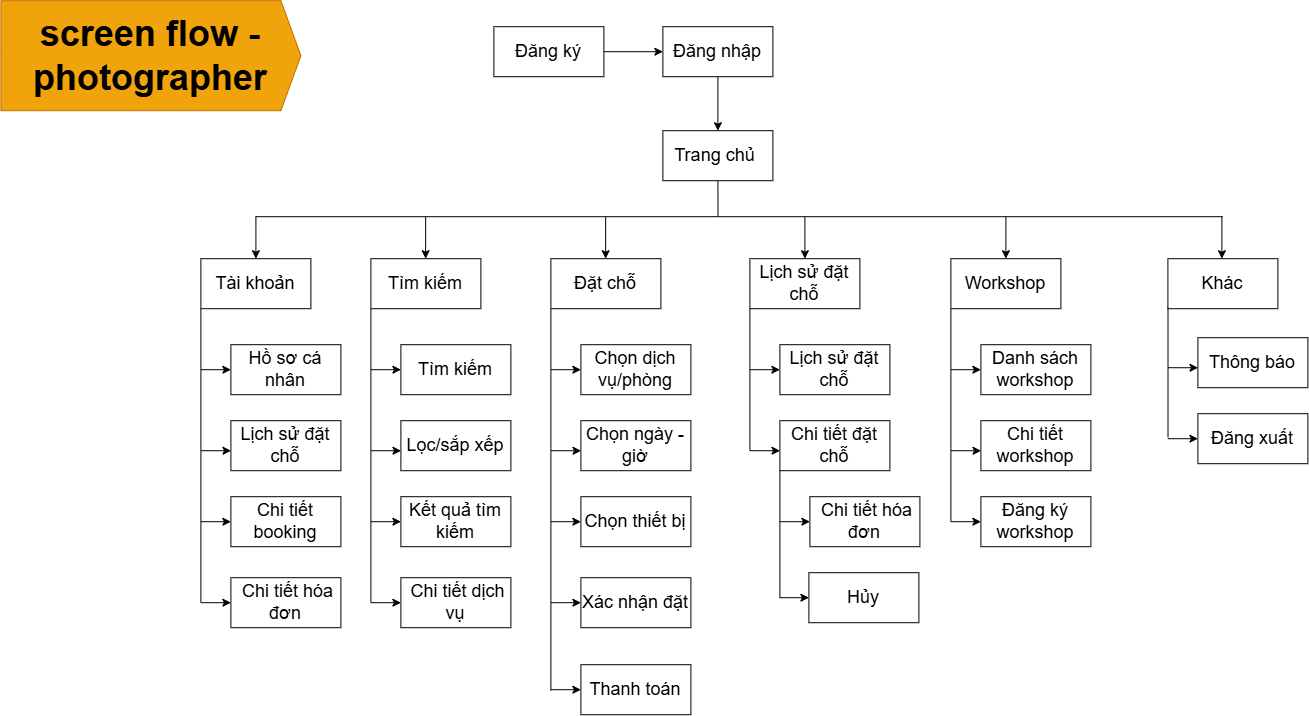
\includegraphics[width=\textwidth]{images/4.png}
	\caption{Screen Flow của Photographer}
	\label{fig:screen-flow-photographer}
\end{figure}

\begin{figure}[H]
	\centering
	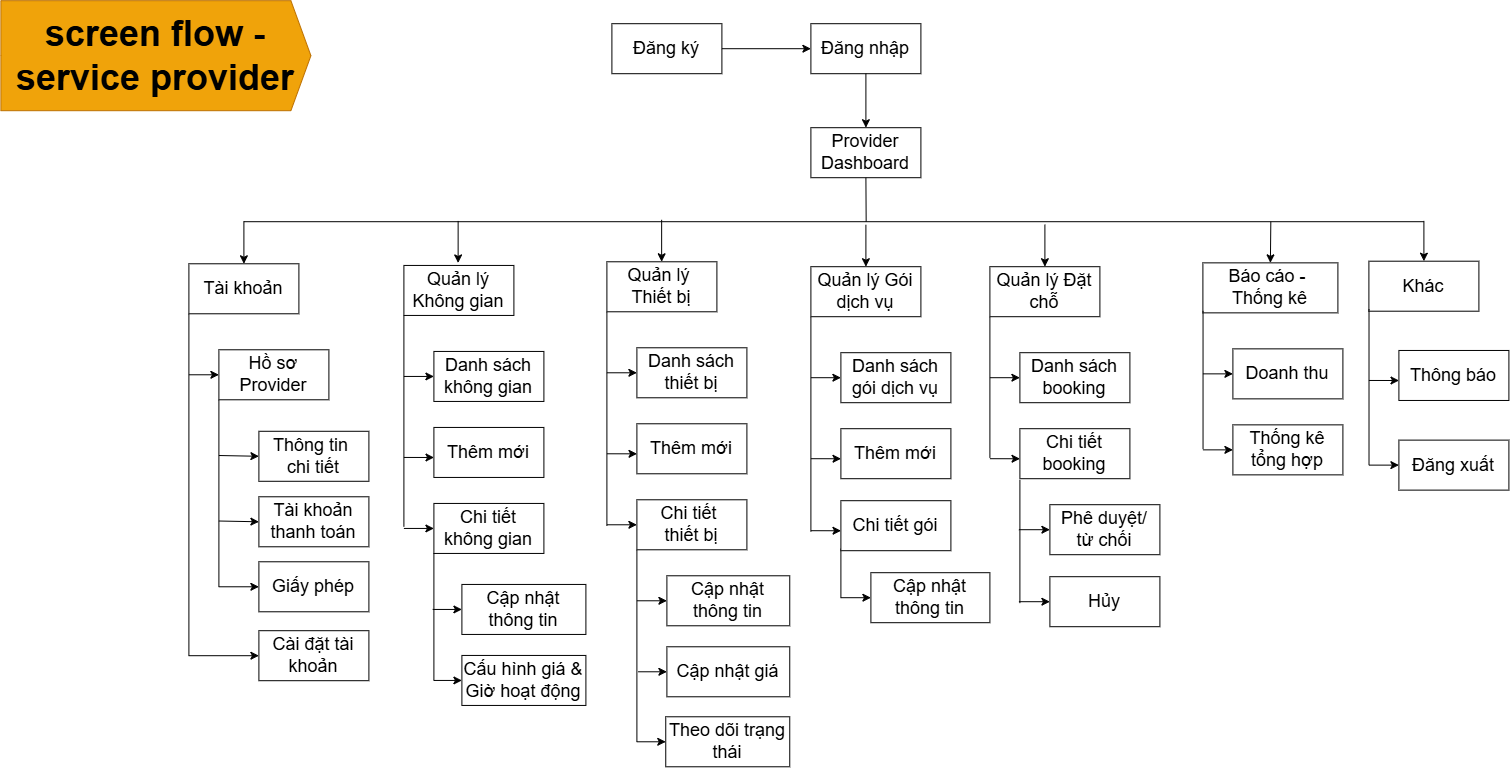
\includegraphics[width=\textwidth]{images/5.png}
	\caption{Screen Flow của Service Provider}
	\label{fig:screen-flow-provider}
\end{figure}

\begin{figure}[H]
	\centering
	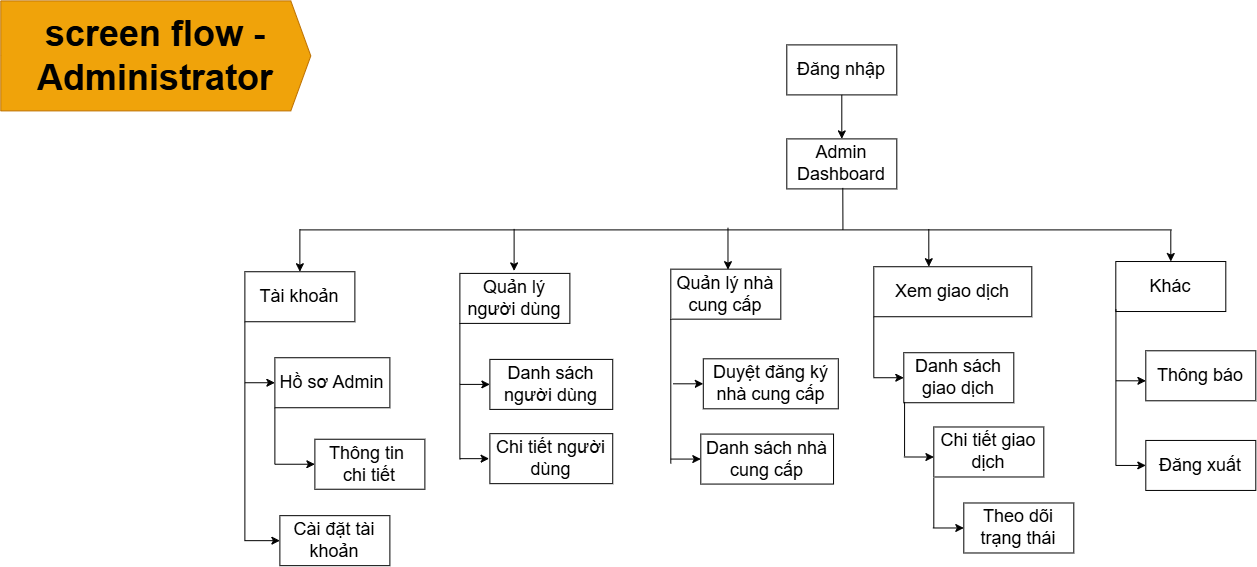
\includegraphics[width=\textwidth]{images/6.png}
	\caption{Screen Flow của Administrator}
	\label{fig:screen-flow-admin}
\end{figure}


\subsubsection{Mô tả màn hình}

\textbf{Nhóm màn hình dùng chung}

\begin{table}[H]
	\centering
	\caption{Các màn hình dùng chung}
	\label{tab:common-screens}
	\begin{tabular}{|c|p{3cm}|p{3cm}|p{5cm}|}
		\hline
		\textbf{\#} & \textbf{Nhóm} & \textbf{Màn hình} & \textbf{Mô tả} \\
		\hline
		
		1 & Xác thực & Đăng nhập &
		Cho phép người dùng đăng nhập vào hệ thống. \\
		\hline
		
		2 & Xác thực & Đăng ký &
		Cho phép Photographer và Service Provider tạo tài khoản. \\
		\hline
		
		3 & Xác thực & Đăng xuất &
		Kết thúc phiên đăng nhập hiện tại. \\
		\hline
	
	\end{tabular}
\end{table}


\textbf{Nhóm màn hình Photographer}

% =========================================================
% CÁC MÀN HÌNH PHOTOGRAPHER
% =========================================================

\setlength{\LTleft}{0pt}
\setlength{\LTright}{0pt}
\renewcommand{\arraystretch}{1.3}

\begin{longtable}{|p{0.8cm}|p{2.5cm}|p{3.2cm}|p{5.0cm}|}
	
	\caption{\raggedright Các màn hình Photographer}
	\label{tab:photographer-screens}\\
	
	\hline
	
	\textbf{\#} &
	\textbf{Nhóm} &
	\textbf{Màn hình} &
	\textbf{Mô tả} \\
	
	\hline
	\endfirsthead
	
	\hline
	
	\textbf{\#} &
	\textbf{Nhóm} &
	\textbf{Màn hình} &
	\textbf{Mô tả} \\
	
	\hline
	\endhead
	
	1 &
	Trang chủ &
	Trang chủ Photographer &
	Hiển thị tổng quan và các chức năng chính. \\
	
	\hline
	
	2 &
	Tìm kiếm &
	Tìm kiếm dịch vụ &
	Cho phép tìm kiếm Creative Space và dịch vụ. \\
	
	\hline
	
	3 &
	Tìm kiếm &
	Kết quả tìm kiếm &
	Hiển thị danh sách dịch vụ phù hợp với yêu cầu tìm kiếm. \\
	
	\hline
	
	4 &
	Tìm kiếm &
	Chi tiết dịch vụ &
	Hiển thị thông tin chi tiết của Creative Space hoặc dịch vụ. \\
	
	\hline
	
	5 &
	Booking &
	Chọn dịch vụ/không gian &
	Cho phép lựa chọn dịch vụ hoặc không gian cần đặt. \\
	
	\hline
	
	6 &
	Booking &
	Chọn ngày và giờ &
	Cho phép lựa chọn thời gian sử dụng dịch vụ. \\
	
	\hline
	
	7 &
	Booking &
	Chọn thiết bị &
	Cho phép lựa chọn thiết bị đi kèm nếu có. \\
	
	\hline
	
	8 &
	Booking &
	Xác nhận đặt chỗ &
	Hiển thị thông tin Booking trước khi xác nhận. \\
	
	\hline
	
	9 &
	Booking &
	Chi tiết Booking &
	Hiển thị thông tin chi tiết của Booking. \\
	
	\hline
	
	10 &
	Booking &
	Hủy Booking &
	Cho phép người dùng hủy Booking phù hợp. \\
	
	\hline
	
	11 &
	Booking &
	Lịch sử Booking &
	Hiển thị danh sách các Booking đã thực hiện. \\
	
	\hline
	
	12 &
	Thanh toán &
	Thanh toán &
	Hiển thị thông tin và trạng thái thanh toán. \\
	
	\hline
	
	13 &
	Hóa đơn &
	Chi tiết hóa đơn &
	Hiển thị thông tin hóa đơn của Booking. \\
	
	\hline
	
	14 &
	Workshop &
	Danh sách Workshop &
	Hiển thị danh sách Workshop. \\
	
	\hline
	
	15 &
	Workshop &
	Chi tiết Workshop &
	Hiển thị thông tin chi tiết Workshop. \\
	
	\hline
	
	16 &
	Workshop &
	Đăng ký Workshop &
	Cho phép Photographer đăng ký Workshop. \\
	
	\hline
	
	17 &
	Hồ sơ &
	Hồ sơ cá nhân &
	Cho phép Photographer xem và cập nhật thông tin cá nhân. \\
	
	\hline
	
	18 &
	Tài khoản &
	Đổi mật khẩu &
	Cho phép Photographer thay đổi mật khẩu. \\
	
	\hline
	
	19 &
	Thông báo &
	Thông báo &
	Hiển thị các thông báo của Photographer. \\
	
	\hline
	
\end{longtable}

\setlength{\LTleft}{0pt}
\setlength{\LTright}{0pt}
\renewcommand{\arraystretch}{1.3}


\textbf{Nhóm màn hình Service Provider}

\setlength{\LTleft}{0pt}
\setlength{\LTright}{0pt}
\renewcommand{\arraystretch}{1.3}

\begin{longtable}{|p{0.8cm}|p{2.5cm}|p{3.2cm}|p{5.0cm}|}
	
	\caption{\raggedright Các màn hình Service Provider}
	\label{tab:provider-screens}\\
	
	\hline
	
	\textbf{\#} &
	\textbf{Nhóm} &
	\textbf{Màn hình} &
	\textbf{Mô tả} \\
	
	\hline
	\endfirsthead
	
	\hline
	
	\textbf{\#} &
	\textbf{Nhóm} &
	\textbf{Màn hình} &
	\textbf{Mô tả} \\
	
	\hline
	\endhead
	
	1 &
	Dashboard &
	Provider Dashboard &
	Hiển thị tổng quan hoạt động của Provider. \\
	
	\hline
	
	2 &
	Hồ sơ &
	Hồ sơ Provider &
	Xem và cập nhật thông tin Provider. \\
	
	\hline
	
	3 &
	Không gian &
	Danh sách không gian &
	Hiển thị các Creative Space do Provider quản lý. \\
	
	\hline
	
	4 &
	Không gian &
	Thêm/Cập nhật không gian &
	Thêm hoặc cập nhật thông tin Creative Space. \\
	
	\hline
	
	5 &
	Thiết bị &
	Danh sách thiết bị &
	Hiển thị các thiết bị Provider quản lý. \\
	
	\hline
	
	6 &
	Thiết bị &
	Thêm/Cập nhật thiết bị &
	Thêm hoặc cập nhật thông tin thiết bị. \\
	
	\hline
	
	7 &
	Gói dịch vụ &
	Danh sách gói dịch vụ &
	Hiển thị các Service Package. \\
	
	\hline
	
	8 &
	Gói dịch vụ &
	Thêm/Cập nhật gói dịch vụ &
	Thêm hoặc cập nhật thông tin Service Package. \\
	
	\hline
	
	9 &
	Booking &
	Danh sách Booking &
	Hiển thị các Booking được gửi đến Provider. \\
	
	\hline
	
	10 &
	Booking &
	Chi tiết Booking &
	Hiển thị thông tin chi tiết Booking. \\
	
	\hline
	
	11 &
	Booking &
	Xác nhận/Từ chối &
	Cho phép Provider xử lý yêu cầu Booking. \\
	
	\hline
	
	12 &
	Booking &
	Check-in/Check-out &
	Xác nhận quá trình sử dụng dịch vụ. \\
	
	\hline
	
	13 &
	Workshop &
	Quản lý Workshop &
	Tạo và quản lý Workshop. \\
	
	\hline
	
	14 &
	Workshop &
	Người đăng ký &
	Hiển thị danh sách người đăng ký Workshop. \\
	
	\hline
	
	15 &
	Thanh toán &
	Thông tin thanh toán &
	Theo dõi thông tin thanh toán của Booking. \\
	
	\hline
	
	16 &
	Thông báo &
	Thông báo &
	Hiển thị thông báo cho Provider. \\
	
	\hline
	
\end{longtable}

\setlength{\LTleft}{0pt}
\setlength{\LTright}{0pt}
\renewcommand{\arraystretch}{1.3}


\textbf{Nhóm màn hình Administrator}

\setlength{\LTleft}{0pt}
\setlength{\LTright}{0pt}
\renewcommand{\arraystretch}{1.3}

\begin{longtable}{
		|>{\raggedright\arraybackslash}p{0.8cm}|
		>{\raggedright\arraybackslash}p{2.5cm}|
		>{\raggedright\arraybackslash}p{3.2cm}|
		>{\raggedright\arraybackslash}p{5.0cm}|
	}
	
	\caption{\raggedright Các màn hình Administrator}
	\label{tab:admin-screens}\\
	
	\hline
	
	\textbf{\#} &
	\textbf{Nhóm} &
	\textbf{Màn hình} &
	\textbf{Mô tả} \\
	
	\hline
	\endfirsthead
	
	\hline
	
	\textbf{\#} &
	\textbf{Nhóm} &
	\textbf{Màn hình} &
	\textbf{Mô tả} \\
	
	\hline
	\endhead
	
	1 &
	Dashboard &
	Admin Dashboard &
	Hiển thị tổng quan hoạt động quản trị. \\
	
	\hline
	
	2 &
	Người dùng &
	Danh sách người dùng &
	Hiển thị danh sách người dùng. \\
	
	\hline
	
	3 &
	Người dùng &
	Chi tiết người dùng &
	Hiển thị thông tin chi tiết người dùng. \\
	
	\hline
	
	4 &
	Provider &
	Danh sách Provider &
	Hiển thị danh sách Service Provider. \\
	
	\hline
	
	5 &
	Provider &
	Chi tiết Provider &
	Hiển thị thông tin chi tiết Service Provider. \\
	
	\hline
	
	6 &
	Phê duyệt &
	Danh sách đăng ký Provider &
	Hiển thị các đăng ký Service Provider cần xử lý. \\
	
	\hline
	
	7 &
	Phê duyệt &
	Phê duyệt Provider &
	Cho phép Administrator phê duyệt Service Provider. \\
	
	\hline
	
	8 &
	Giao dịch &
	Danh sách giao dịch &
	Hiển thị các giao dịch trong hệ thống. \\
	
	\hline
	
	9 &
	Giao dịch &
	Chi tiết giao dịch &
	Hiển thị thông tin chi tiết giao dịch. \\
	
	\hline
	
	10 &
	Hồ sơ &
	Hồ sơ Administrator &
	Cho phép Administrator xem và cập nhật thông tin tài khoản. \\
	
	\hline
	
	11 &
	Thông báo &
	Thông báo &
	Hiển thị các thông báo của Administrator. \\
	
	\hline
	
\end{longtable}

\setlength{\LTleft}{0pt}
\setlength{\LTright}{0pt}
\renewcommand{\arraystretch}{1.3}


\subsubsection{Phân quyền màn hình}

Hệ thống phân quyền màn hình dựa trên vai trò của người dùng. Mỗi màn hình
được giới hạn quyền truy cập tương ứng với vai trò Photographer,
Service Provider hoặc Administrator nhằm đảm bảo người dùng chỉ có thể
sử dụng các chức năng phù hợp với quyền hạn của mình.

\setlength{\LTleft}{0pt}
\setlength{\LTright}{0pt}
\renewcommand{\arraystretch}{1.3}

\begin{longtable}{|>{\raggedright\arraybackslash}p{3.0cm}|c|c|c|}
	
	\caption{\raggedright Phân quyền màn hình theo vai trò}
	\label{tab:authorization}\\
	
	\hline
	
	\textbf{Màn hình} &
	\textbf{Photographer} &
	\textbf{Service Provider} &
	\textbf{Administrator} \\
	
	\hline
	\endfirsthead
	
	\hline
	\textbf{Màn hình} &
	\textbf{Photographer} &
	\textbf{Service Provider} &
	\textbf{Administrator} \\
	\hline
	\endhead
	
	Đăng nhập &
	$\checkmark$ &
	$\checkmark$ &
	$\checkmark$ \\ \hline
	
	Đăng ký tài khoản &
	$\checkmark$ &
	$\checkmark$ &
	\\ \hline
	
	Đăng xuất &
	$\checkmark$ &
	$\checkmark$ &
	$\checkmark$ \\ \hline
	
	Trang chủ &
	$\checkmark$ &
	$\checkmark$ &
	$\checkmark$ \\ \hline
	
	Tìm kiếm dịch vụ &
	$\checkmark$ &
	&
	\\ \hline
	
	Kết quả tìm kiếm &
	$\checkmark$ &
	&
	\\ \hline
	
	Chi tiết Creative Space &
	$\checkmark$ &
	&
	\\ \hline
	
	Chọn dịch vụ/không gian Booking &
	$\checkmark$ &
	&
	\\ \hline
	
	Chọn ngày và giờ Booking &
	$\checkmark$ &
	&
	\\ \hline
	
	Chọn thiết bị &
	$\checkmark$ &
	&
	\\ \hline
	
	Xác nhận Booking &
	$\checkmark$ &
	&
	\\ \hline
	
	Chi tiết Booking &
	$\checkmark$ &
	$\checkmark$ &
	\\ \hline
	
	Hủy Booking &
	$\checkmark$ &
	&
	\\ \hline
	
	Lịch sử Booking &
	$\checkmark$ &
	&
	\\ \hline
	
	Thanh toán &
	$\checkmark$ &
	$\checkmark$ &
	$\checkmark$ \\ \hline
	
	Chi tiết hóa đơn &
	$\checkmark$ &
	&
	\\ \hline
	
	Danh sách Workshop &
	$\checkmark$ &
	$\checkmark$ &
	\\ \hline
	
	Chi tiết Workshop &
	$\checkmark$ &
	$\checkmark$ &
	\\ \hline
	
	Đăng ký Workshop &
	$\checkmark$ &
	&
	\\ \hline
	
	Hồ sơ Photographer &
	$\checkmark$ &
	&
	\\ \hline
	
	Hồ sơ Service Provider &
	&
	$\checkmark$ &
	\\ \hline
	
	Đổi mật khẩu &
	$\checkmark$ &
	$\checkmark$ &
	$\checkmark$ \\ \hline
	
	Thông báo Photographer &
	$\checkmark$ &
	&
	\\ \hline
	
	Thông báo Service Provider &
	&
	$\checkmark$ &
	\\ \hline
	
	Thông báo Administrator &
	&
	&
	$\checkmark$ \\ \hline
	
	Provider Dashboard &
	&
	$\checkmark$ &
	\\ \hline
	
	Quản lý Creative Space &
	&
	$\checkmark$ &
	\\ \hline
	
	Quản lý thiết bị &
	&
	$\checkmark$ &
	\\ \hline
	
	Quản lý gói dịch vụ &
	&
	$\checkmark$ &
	\\ \hline
	
	Quản lý Booking &
	&
	$\checkmark$ &
	\\ \hline
	
	Xác nhận/Từ chối Booking &
	&
	$\checkmark$ &
	\\ \hline
	
	Check-in/Check-out &
	&
	$\checkmark$ &
	\\ \hline
	
	Quản lý Workshop &
	&
	$\checkmark$ &
	\\ \hline
	
	Người đăng ký Workshop &
	&
	$\checkmark$ &
	\\ \hline
	
	Thông tin thanh toán Provider &
	&
	$\checkmark$ &
	\\ \hline
	
	Quản lý người dùng &
	&
	&
	$\checkmark$ \\ \hline
	
	Quản lý Provider &
	&
	&
	$\checkmark$ \\ \hline
	
	Phê duyệt Provider &
	&
	&
	$\checkmark$ \\ \hline
	
	Quản lý giao dịch &
	&
	&
	$\checkmark$ \\ \hline
	
\end{longtable}

\setlength{\LTleft}{0pt}
\setlength{\LTright}{0pt}
\renewcommand{\arraystretch}{1.3}


\subsubsection{Chức năng không thông qua màn hình}

Một số chức năng của hệ thống được thực hiện tự động ở phía Backend mà
không yêu cầu người dùng thao tác trực tiếp trên một màn hình riêng biệt.
Các chức năng này hỗ trợ xác thực, xử lý thông tin đặt chỗ, thanh toán,
quản lý trạng thái và gửi thông báo trong quá trình vận hành hệ thống.
Bảng dưới đây tổng hợp các chức năng không thông qua màn hình được triển
khai trong hệ thống.

\setlength{\LTleft}{0pt}
\setlength{\LTright}{0pt}
\renewcommand{\arraystretch}{1.3}

\begin{longtable}{
		|>{\raggedright\arraybackslash}p{0.8cm}|
		>{\raggedright\arraybackslash}p{3.0cm}|
		>{\raggedright\arraybackslash}p{3.0cm}|
		>{\raggedright\arraybackslash}p{4.7cm}|
	}
	
	\caption{\raggedright Các chức năng không thông qua màn hình}
	\label{tab:non-screen}\\
	
	\hline
	
	\textbf{\#} &
	\textbf{Chức năng} &
	\textbf{Module} &
	\textbf{Mô tả} \\
	
	\hline
	\endfirsthead
	
	\hline
	
	\textbf{\#} &
	\textbf{Chức năng} &
	\textbf{Module} &
	\textbf{Mô tả} \\
	
	\hline
	\endhead
	
	1 &
	Xác thực tài khoản &
	Authentication &
	Xử lý xác thực thông tin tài khoản và trạng thái tài khoản trong quá trình đăng nhập và truy cập các chức năng yêu cầu xác thực. \\
	
	\hline
	
	2 &
	Xác thực OTP &
	Authentication &
	Xử lý mã OTP phục vụ các chức năng xác thực tài khoản, đặc biệt trong quá trình quên mật khẩu và đặt lại mật khẩu. \\
	
	\hline
	
	3 &
	Kiểm tra quyền truy cập &
	Authorization &
	Kiểm tra vai trò của người dùng và xác định quyền thực hiện các chức năng tương ứng trong hệ thống. \\
	
	\hline
	
	4 &
	Kiểm tra khả dụng Booking &
	Booking &
	Kiểm tra thông tin Creative Space, thiết bị và thời gian được lựa chọn trước khi xử lý yêu cầu Booking. \\
	
	\hline
	
	5 &
	Tính tổng chi phí Booking &
	Booking &
	Tự động tính toán tổng chi phí dựa trên các dịch vụ, Creative Space và thiết bị được lựa chọn trong Booking. \\
	
	\hline
	
	6 &
	Cập nhật trạng thái Booking &
	Booking &
	Tự động cập nhật trạng thái Booking theo quá trình xử lý như xác nhận, từ chối, hủy, check-in và check-out. \\
	
	\hline
	
	7 &
	Xử lý thanh toán &
	Payment &
	Xử lý thông tin thanh toán và cập nhật trạng thái thanh toán tương ứng với Booking. \\
	
	\hline
	
	8 &
	Tạo hóa đơn &
	Invoice &
	Tạo thông tin hóa đơn tương ứng với Booking và lưu trữ thông tin hóa đơn trong hệ thống. \\
	
	\hline
	
	9 &
	Kiểm tra trạng thái Provider &
	Service Provider &
	Kiểm tra trạng thái phê duyệt của Service Provider để xác định Provider có đủ điều kiện cung cấp dịch vụ trên hệ thống hay không. \\
	
	\hline
	
	10 &
	Xử lý đăng ký Workshop &
	Workshop &
	Xử lý thông tin đăng ký Workshop và cập nhật thông tin đăng ký của Photographer trong hệ thống. \\
	
	\hline
	
	11 &
	Gửi thông báo &
	Notification &
	Tạo và gửi thông báo đến người dùng liên quan khi phát sinh các sự kiện trong quá trình sử dụng hệ thống. \\
	
	\hline
	
\end{longtable}

\setlength{\LTleft}{0pt}
\setlength{\LTright}{0pt}
\renewcommand{\arraystretch}{1.3}


\subsubsection{Sơ đồ quan hệ thực thể}

Sơ đồ quan hệ thực thể mô tả các thực thể chính trong hệ thống và mối
quan hệ giữa các thực thể.

\begin{figure}[H]
	\centering
	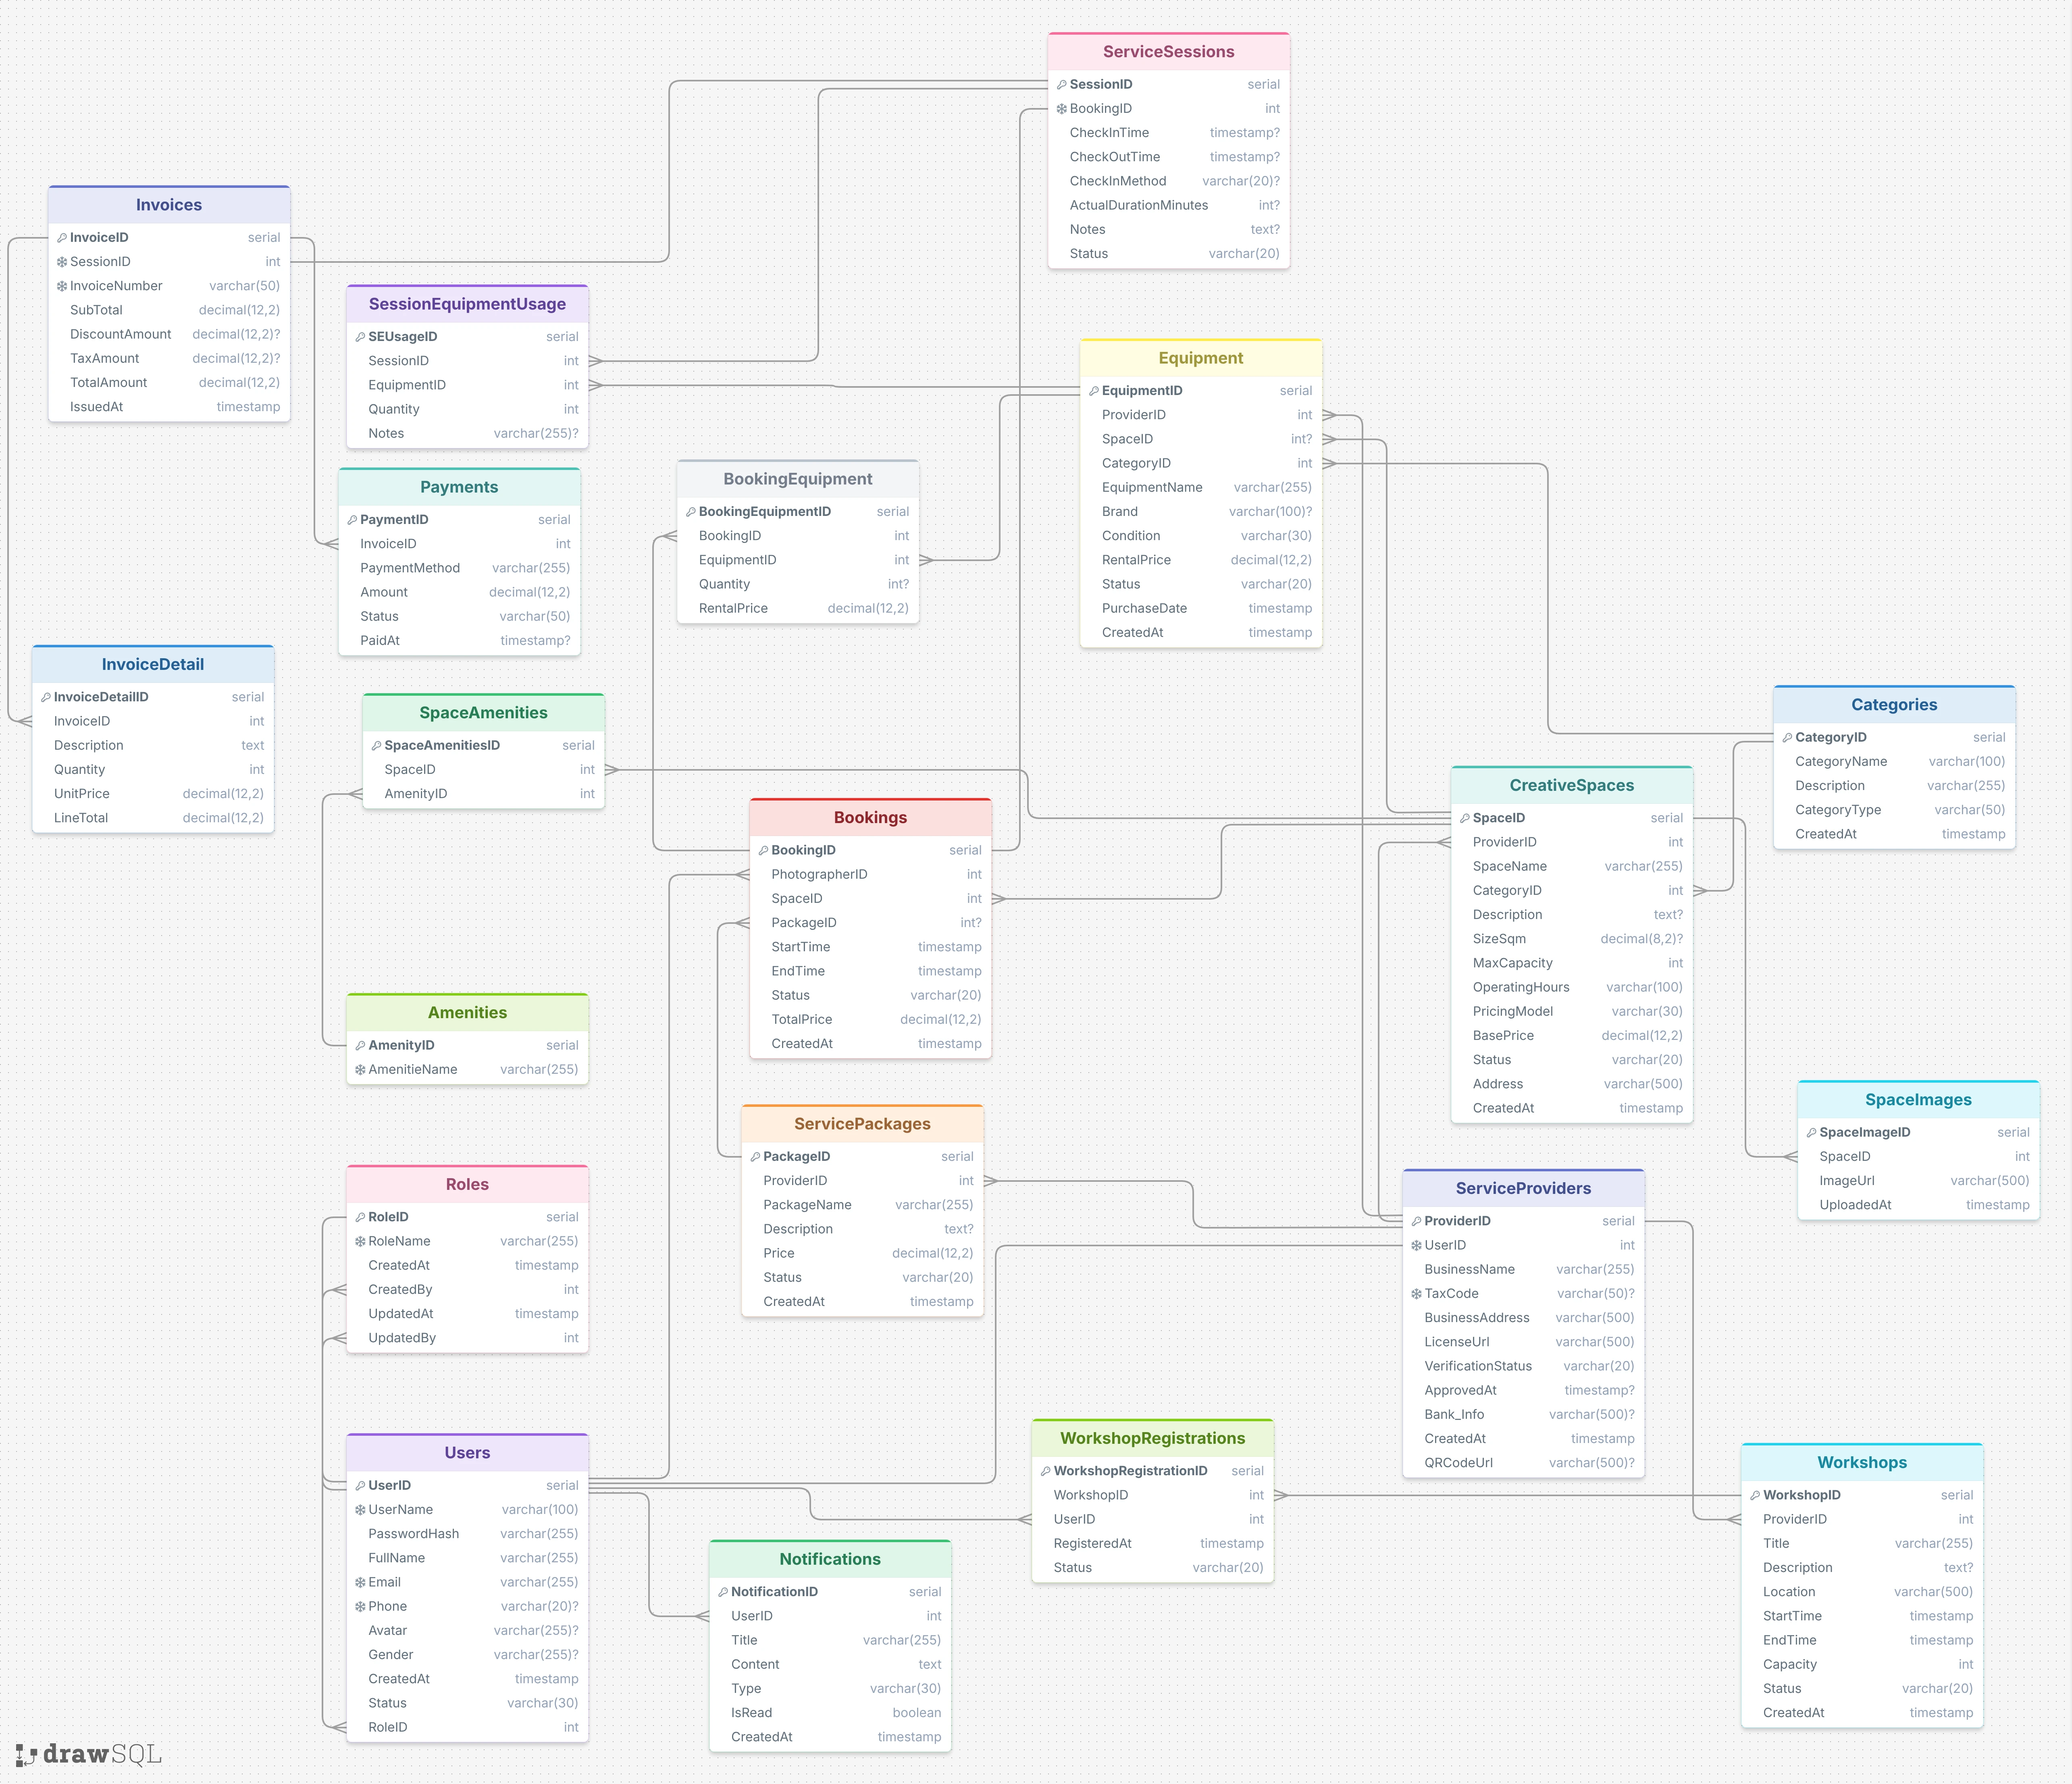
\includegraphics[width=\textwidth]{images/7.png}
	\caption{Sơ đồ quan hệ thực thể của hệ thống}
	\label{fig:erd}
\end{figure}


% =========================================================
% 3.2 XÁC THỰC
% =========================================================

\subsection{Xác thực}

Chức năng xác thực chịu trách nhiệm xác thực người dùng trước khi cho
phép truy cập vào hệ thống.

\subsubsection{Đăng nhập}

Người dùng nhập thông tin tài khoản để đăng nhập.

Hệ thống kiểm tra thông tin đăng nhập và trạng thái tài khoản. Nếu thông
tin hợp lệ, hệ thống chuyển người dùng đến Dashboard tương ứng với vai
trò. Nếu thông tin không hợp lệ, hệ thống hiển thị thông báo lỗi.

\subsubsection{Đăng ký}

Photographer và Service Provider có thể đăng ký tài khoản mới trên hệ
thống.

Sau khi đăng ký thành công, thông tin tài khoản được lưu vào hệ thống.

\subsubsection{Đăng xuất}

Người dùng có thể đăng xuất để kết thúc phiên làm việc hiện tại.


% =========================================================
% 3.3 QUẢN LÝ PHOTOGRAPHER
% =========================================================

\subsection{Quản lý Photographer}

Chức năng quản lý Photographer cho phép người dùng quản lý thông tin
tài khoản và hồ sơ cá nhân.

\subsubsection{Quản lý hồ sơ Photographer}

Photographer có thể xem và cập nhật thông tin cá nhân của mình.

Thông tin được cập nhật sẽ được lưu lại để sử dụng trong các chức năng
khác của hệ thống.

\subsubsection{Quên mật khẩu}

Photographer có thể yêu cầu khôi phục mật khẩu khi không nhớ mật khẩu
đăng nhập.

Hệ thống thực hiện quy trình xác thực cần thiết và cho phép người dùng
thiết lập mật khẩu mới.

\subsubsection{Đổi mật khẩu}

Photographer đã đăng nhập có thể thay đổi mật khẩu tài khoản.


% =========================================================
% 3.4 TÌM KIẾM VÀ KHÁM PHÁ DỊCH VỤ
% =========================================================

\subsection{Tìm kiếm và khám phá dịch vụ}

Chức năng này hỗ trợ Photographer tìm kiếm và khám phá các dịch vụ
phòng tối, studio và các tài nguyên được cung cấp trên nền tảng.

\subsubsection{Tìm kiếm dịch vụ}

Photographer nhập thông tin tìm kiếm để tìm các creative space hoặc
dịch vụ phù hợp.

Hệ thống trả về danh sách các kết quả phù hợp với thông tin tìm kiếm.

\subsubsection{Lọc và sắp xếp dịch vụ}

Photographer có thể lọc và sắp xếp danh sách kết quả dựa trên các tiêu
chí được hệ thống hỗ trợ.

\subsubsection{Xem chi tiết dịch vụ}

Photographer có thể chọn một dịch vụ trong danh sách để xem thông tin
chi tiết trước khi thực hiện booking.


% =========================================================
% 3.5 QUẢN LÝ ĐẶT CHỖ
% =========================================================

\subsection{Quản lý đặt chỗ}

Chức năng quản lý đặt chỗ hỗ trợ Photographer thực hiện quá trình lựa
chọn dịch vụ và tạo booking.

\subsubsection{Chọn dịch vụ/không gian}

Photographer lựa chọn creative space hoặc dịch vụ cần sử dụng.

\subsubsection{Chọn ngày và giờ}

Photographer lựa chọn ngày và khoảng thời gian sử dụng dịch vụ.

Hệ thống kiểm tra khả dụng của khoảng thời gian được lựa chọn.

\subsubsection{Chọn thiết bị}

Photographer có thể lựa chọn thiết bị đi kèm nếu dịch vụ hỗ trợ.

\subsubsection{Xác nhận booking}

Hệ thống hiển thị thông tin dịch vụ, thời gian, thiết bị và chi phí để
Photographer kiểm tra trước khi xác nhận booking.

\subsubsection{Hủy booking}

Photographer có thể hủy booking phù hợp với trạng thái hiện tại của
booking.

\subsubsection{Check-in/Check-out}

Hệ thống hỗ trợ ghi nhận trạng thái bắt đầu và kết thúc sử dụng dịch vụ
thông qua chức năng check-in và check-out.


% =========================================================
% 3.6 THANH TOÁN VÀ QUẢN LÝ BOOKING
% =========================================================

\subsection{Thanh toán và quản lý booking}

Chức năng này hỗ trợ Photographer theo dõi booking và thực hiện các
nghiệp vụ liên quan đến thanh toán.

\subsubsection{Thanh toán}

Photographer thực hiện thanh toán cho booking thông qua phương thức thanh
toán được hệ thống hỗ trợ.

Sau khi thanh toán được xử lý, hệ thống cập nhật trạng thái thanh toán
và booking.

\subsubsection{Xem lịch sử booking}

Photographer có thể xem danh sách các booking đã thực hiện.

Lịch sử booking giúp người dùng theo dõi các lần đặt chỗ trước đó.

\subsubsection{Xem chi tiết booking}

Photographer có thể xem thông tin chi tiết của từng booking bao gồm
dịch vụ, thời gian, chi phí và trạng thái booking.

\subsubsection{Xem hóa đơn}

Photographer có thể xem thông tin hóa đơn tương ứng với booking.


% =========================================================
% 3.7 QUẢN LÝ WORKSHOP
% =========================================================

\subsection{Quản lý Workshop}

Chức năng Workshop hỗ trợ Photographer xem và đăng ký các workshop được
tổ chức trên nền tảng.

\subsubsection{Xem danh sách Workshop}

Photographer có thể truy cập danh sách các workshop đang được tổ chức
trên hệ thống.

Danh sách workshop hiển thị các thông tin cơ bản giúp người dùng lựa
chọn workshop phù hợp.

\subsubsection{Xem chi tiết Workshop}

Photographer có thể chọn một workshop để xem thông tin chi tiết.

Thông tin chi tiết bao gồm các thông tin được Provider cung cấp như tên
workshop, nội dung, thời gian và các thông tin liên quan.

\subsubsection{Đăng ký Workshop}

Photographer có thể đăng ký tham gia workshop.

Hệ thống kiểm tra thông tin đăng ký và lưu thông tin tham gia workshop
của Photographer.


% =========================================================
% 3.8 QUẢN LÝ SERVICE PROVIDER
% =========================================================

\subsection{Quản lý Service Provider}

Chức năng quản lý Service Provider hỗ trợ Provider quản lý các hoạt động
cung cấp dịch vụ trên nền tảng.

\subsubsection{Quản lý không gian}

Service Provider có thể thêm, cập nhật và quản lý thông tin các creative
space thuộc quyền quản lý của mình.

\subsubsection{Quản lý thiết bị}

Service Provider có thể thêm, cập nhật và quản lý các thiết bị được cung
cấp trên nền tảng.

\subsubsection{Quản lý gói dịch vụ}

Service Provider có thể tạo và cập nhật các service package.

Thông tin gói dịch vụ được sử dụng khi Photographer tìm kiếm và đặt
dịch vụ.

\subsubsection{Quản lý booking}

Service Provider có thể xem danh sách booking được gửi đến mình.

Provider có thể xem thông tin chi tiết của từng booking để xử lý.

\subsubsection{Xác nhận hoặc từ chối booking}

Service Provider có thể xác nhận hoặc từ chối yêu cầu booking từ
Photographer.

Sau khi xử lý, trạng thái booking được cập nhật trong hệ thống.

\subsubsection{Check-in/Check-out}

Service Provider có thể thực hiện hoặc ghi nhận trạng thái check-in và
check-out của booking.

Chức năng này giúp xác định quá trình sử dụng dịch vụ của Photographer.

\subsubsection{Quản lý Workshop}

Service Provider có thể tạo và quản lý các workshop do mình tổ chức.

Provider có thể cập nhật thông tin workshop để Photographer xem và đăng
ký tham gia.

\subsubsection{Xem người đăng ký Workshop}

Service Provider có thể xem danh sách Photographer đã đăng ký tham gia
một workshop.

Thông tin này giúp Provider theo dõi số lượng người tham gia.

\subsubsection{Quản lý hồ sơ Provider}

Service Provider có thể xem và cập nhật thông tin hồ sơ của mình.

\subsubsection{Xem Dashboard}

Service Provider có thể xem Dashboard để theo dõi tổng quan hoạt động
của mình trên hệ thống.

\subsubsection{Quản lý thông tin thanh toán}

Service Provider có thể xem thông tin thanh toán liên quan đến các
booking được thực hiện trên nền tảng.


% =========================================================
% 3.9 QUẢN LÝ ADMINISTRATOR
% =========================================================

\subsection{Quản lý Administrator}

Administrator chịu trách nhiệm quản lý các thông tin và hoạt động quản
trị chính của hệ thống.

\subsubsection{Quản lý người dùng}

Administrator có thể xem danh sách và thông tin người dùng trên hệ thống.

\subsubsection{Quản lý Service Provider}

Administrator có thể xem và quản lý thông tin các Service Provider.

\subsubsection{Phê duyệt Service Provider}

Administrator có thể xem các đăng ký Service Provider và thực hiện phê
duyệt.

Chỉ Service Provider được phê duyệt mới có thể thực hiện các hoạt động
cung cấp dịch vụ theo quy định của hệ thống.

\subsubsection{Quản lý giao dịch}

Administrator có thể xem danh sách và thông tin các giao dịch trên hệ
thống để theo dõi hoạt động thanh toán.


% =========================================================
% 3.10 QUẢN LÝ THÔNG BÁO
% =========================================================

\subsection{Quản lý thông báo}

Hệ thống cung cấp chức năng thông báo cho Photographer, Service Provider
và Administrator.

\subsubsection{Xem thông báo}

Người dùng có thể xem danh sách các thông báo liên quan đến hoạt động
của tài khoản.

Thông báo có thể liên quan đến booking, thanh toán, phê duyệt Provider
hoặc các thay đổi trạng thái khác trong hệ thống.


% =========================================================
% 4. YÊU CẦU PHI CHỨC NĂNG
% =========================================================

\section{Yêu cầu phi chức năng}


\subsection{Giao diện bên ngoài}

Hệ thống cung cấp các giao diện bên ngoài phục vụ người dùng và các
hoạt động nghiệp vụ chính.

\begin{itemize}
	\item \textbf{Giao diện người dùng:} cung cấp giao diện web cho ba
	nhóm người dùng gồm Photographer, Service Provider và Administrator.
	
	\item \textbf{Giao diện thanh toán:} cung cấp giao diện để
	Photographer thực hiện thanh toán cho Booking thông qua
	QR/chuyển khoản ngân hàng và theo dõi trạng thái thanh toán.
	
	\item \textbf{Giao diện thông báo:} cung cấp giao diện hiển thị
	các thông báo liên quan đến hoạt động của hệ thống cho
	Photographer, Service Provider và Administrator.
\end{itemize}


\subsection{Thuộc tính chất lượng}

\begin{itemize}
	
	\item \textbf{Bảo mật:} hệ thống phải xác thực người dùng và
	kiểm soát quyền truy cập dựa trên vai trò Photographer,
	Service Provider và Administrator.
	
	\item \textbf{Tính toàn vẹn dữ liệu:} hệ thống phải đảm bảo
	dữ liệu người dùng, Creative Space, Equipment, Service Package,
	Booking, Workshop, thanh toán và hóa đơn được lưu trữ chính xác
	và nhất quán.
	
	\item \textbf{Tính khả dụng:} hệ thống phải cho phép người dùng
	truy cập và sử dụng các chức năng tương ứng với quyền được cấp.
	
	\item \textbf{Khả năng mở rộng:} hệ thống nên có khả năng mở rộng
	để đáp ứng sự gia tăng về số lượng người dùng, Creative Space,
	dịch vụ, Workshop và Booking.
	
	\item \textbf{Khả năng bảo trì:} hệ thống được tổ chức thành các
	module chức năng và các thành phần riêng biệt, giúp thuận tiện
	cho việc bảo trì, sửa lỗi và phát triển thêm chức năng.
	
\end{itemize}


% =========================================================
% 5. PHỤ LỤC YÊU CẦU
% =========================================================
\section{Phụ lục yêu cầu}
\subsection{Quy tắc nghiệp vụ}

\begin{table}[H]
	\centering
	\caption{Các quy tắc nghiệp vụ}
	\label{tab:business-rules}
	\begin{tabular}{|c|p{11cm}|}
		\hline
		\textbf{ID} & \textbf{Quy tắc nghiệp vụ} \\
		\hline
		
		BR-01 &
		Mỗi Photographer chỉ được tạo một tài khoản trên hệ thống. \\
		\hline
		
		BR-02 &
		Service Provider phải được Administrator phê duyệt trước khi
		cung cấp dịch vụ trên nền tảng. \\
		\hline
		
		BR-03 &
		Photographer chỉ có thể đặt Creative Space và các tài nguyên
		đang ở trạng thái khả dụng. \\
		\hline
		
		BR-04 &
		Một Creative Space hoặc Equipment không được phép có các
		booking bị trùng thời gian. \\
		\hline
		
		BR-05 &
		Photographer phải thực hiện thanh toán cho booking theo
		thông tin và trạng thái thanh toán được hệ thống cung cấp. \\
		\hline
		
		BR-06 &
		Service Provider chỉ được quản lý Creative Space, Equipment,
		Service Package, Workshop và Booking thuộc phạm vi của mình. \\
		\hline
		
		BR-07 &
		Chỉ Administrator mới có quyền phê duyệt Service Provider. \\
		\hline
		
		BR-08 &
		Chỉ người dùng đã xác thực mới được truy cập các chức năng
		yêu cầu đăng nhập. \\
		\hline
		
		BR-09 &
		Booking phải được xử lý theo các trạng thái tương ứng trong
		quy trình đặt chỗ và sử dụng dịch vụ. \\
		\hline
		
		BR-10 &
		Check-in và check-out chỉ được thực hiện đối với một Booking
		hợp lệ và có phiên dịch vụ tương ứng. \\
		\hline
		
		BR-11 &
		Một Photographer không được đăng ký trùng một Workshop
		nhiều lần. \\
		\hline
		
		BR-12 &
		Thông báo phải được tạo và hiển thị đến đúng người dùng
		liên quan đến hoạt động của hệ thống. \\
		\hline
		
	\end{tabular}
\end{table}

\subsection{Yêu cầu hệ thống}

\subsubsection{Xác thực và phân quyền}

Hệ thống phải triển khai cơ chế phân quyền dựa trên vai trò (Role-Based
Access Control - RBAC). Người dùng chỉ được phép truy cập các chức năng
phù hợp với vai trò được phân công, bao gồm Photographer, Service Provider
và Administrator.

\subsubsection{Bảo mật dữ liệu}

Thông tin tài khoản, hồ sơ người dùng, thông tin Booking, thanh toán,
hóa đơn và các dữ liệu nghiệp vụ khác phải được bảo vệ thông qua cơ chế
xác thực và kiểm soát quyền truy cập phù hợp.

\subsubsection{Khả năng mở rộng}

Hệ thống phải có khả năng đáp ứng sự gia tăng về số lượng người dùng,
Creative Space, Equipment, Service Package, Workshop và Booking mà không
làm suy giảm đáng kể hiệu năng của hệ thống.

\subsubsection{Tính khả dụng}

Hệ thống cần duy trì khả năng truy cập và sử dụng các chức năng cho
Photographer, Service Provider và Administrator trong thời gian hoạt động
bình thường, ngoại trừ thời gian bảo trì hoặc khi xảy ra sự cố hệ thống.

\subsubsection{Khả năng bảo trì}

Các module của hệ thống phải được tổ chức tương đối độc lập nhằm thuận
tiện cho việc bảo trì, sửa lỗi và phát triển thêm các chức năng trong
tương lai.